\subsection{Installing and invoking Proto-Quipper}

Installation instructions can be found in the README file accompanying the code. 
To build the code type \verb#make# in the main Proto-Quipper directory. 

The \verb#qlib# directory contains some basic modules and examples that can 
be used to test the install. To invoke Proto-Quipper on a file, call 
\begin{verbatim}
./ProtoQuipper qlib/qft.qp -fv
\end{verbatim}
This will run Proto-Quipper on the sample code \verb#qft.qp# and should produce the following output, representing the circuit for the 
Quantum Fourier Transform on three qubits together with its inferred 
type:
\begin{verbatim}
$ ./ProtoQuipper qlib/qft.qp -fv

----------------------*-----*-----H----
                      |     |          
----------*-----H-----|-----R----------
          |           |                
----H-----R-----------R----------------

 : !circ(qubit * qubit * qubit, qubit * qubit * qubit)
\end{verbatim}
The output format is determined by the option provided to \verb#-f#. In the above case, we used \verb#v# to select the visual format. The default format option is \verb#ir#, which outputs the intermediate representation of quantum circuits specified in the context of the QCS program. This output format is compatible with the other tools in the PLATO tool chain, including Quipper.

The \verb#-h# option displays the list of available command line options. 

\subsection{Primitives}

Our implementation of Proto-Quipper was written in Haskell. However, the 
syntax might be more familiar to programmers having experience with OCaml.

Code in Proto-Quipper is organized in modules. Module names always start 
with an upper-case character. The implementation must be placed in a file 
of the same name but written in lower-case and ending with the {\tt.qp} 
extension. For example, the module {\tt List} will be implemented in 
{\tt list.qp}. Modules are organized as follows.
\begin{enumerate}
  \item The module starts with import declarations, e.g., \verb#import Gates ;;#
  \item All the type definitions of the module are placed after the list of imports, e.g., \verb#type list a = Nil | Cons of a * list a ;;#
  \item The rest of the file forms the body of the module, organized as a list of variable declarations and top-level expressions, e.g., \verb#let x = 1 ;;# or \verb#1+1 ;;#
\end{enumerate}

The Proto-Quipper primitives include (most of) the formal syntax presented 
in the preceding sections together with a list of built-in quantum gates. 
Figures \hyperref[types]{\ref*{types}} and \hyperref[terms]{\ref*{terms}} 
describe the correspondence between the formal and implemented versions of 
the core syntax.

\begin{figure}[!ht]
\begin{center}
\renewcommand{\arraystretch}{1.4}
\begin{tabular}{|c|c|}
  \hline
  \textbf{Formalization}    & \textbf{Implementation} \\\hline
  $\qubit$, $\bool$, $1$    & \verb#qubit#, \verb#bool#, \verb#()# \\\hline
  $A \otimes B$             & \verb# A * B# \\\hline
  $A \multimap B$           & \verb# A -> B # \\\hline
  $\Circ(T, U)$              & \verb# circ(T,U)# \\\hline
  ${!} A$                   & \verb# !A# \\\hline
\end{tabular}
\end{center}
\caption{Proto-Quipper Types.}
\label{types}
\end{figure}

\begin{figure}[!ht]
\begin{center}
\renewcommand{\arraystretch}{1.4}
\begin{tabular}{|c|c|}
  \hline
  \textbf{Formalization}          & \textbf{Implementation} \\\hline
  $x$                             & \verb# x# \\\hline
  $\true$, $\false$               & \verb#true#, \verb#false# \\\hline
  $\pair{a}{b}$                   & \verb# (a,b) # \\\hline
  $*$                             & \verb# ()# \\\hline
  $\lambda x.a$                   & \verb# fun x -> a# \\\hline
  $a b$                        & \verb#a b# \\\hline
  $\boxx^T$                       & \verb# box[T]# \\\hline
  $\unbox$, $\rev$                & \verb#unbox#, \verb#rev# \\\hline
  $\ifthenelse{a}{b}{c}$          & \verb# if a then b else c# \\\hline
  $\letin{\p{x,y}}{a}{b}$         & \verb# let (x,y) = a in b# \\\hline
\end{tabular}
\end{center}
\caption{Proto-Quipper Terms.}
\label{terms}
\end{figure}

Note that no term of the form $(t,C,a)$ appears in
Figure~\hyperref[terms]{\ref*{terms}}. This is because the $(t,C,a)$
construct is
not accessible to the programmer. In its place, we provide a set of 
primitive quantum gates. The module \verb#Gates#, which can be found in the 
\verb#qlib# directory, contains a set of basic gates. 
These include: \verb#init0#, \verb#init1#, \verb#term0#, \verb#term1#, 
\verb#not#, \verb#hadamard#, \verb#T#, \verb#S#, \verb#Y#, \verb#Z#, 
\verb#phase#, \verb#W#, \verb#E#, \verb#toffoli#, among others. Please
refer to the documentation for a complete list.

\subsection{Bell states}
\label{ssec-quipper-by-e}

Now that we have introduced the primitive functions that can be used in Proto-Quipper programs, we can combine them into a larger program. We start with 
a basic example: a circuit producing two qubits in the Bell state. Below is
the code of the module \verb#Bell# contained in the file \verb#bell.qp#.

%\begin{figure}[!ht]
\begin{splitcode}
\begin{verbatim}
import Gates

box[] (fun x ->
  let q0 = hadamard (init0 ()) in
  let q1 = init0 () in
  let (q1, q0) = cnot (q1, q0) in
  (q0, q1)
) ;;
\end{verbatim}
  \split \scalebox{1.6}{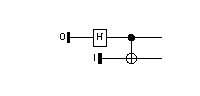
\includegraphics{bell}}
\end{splitcode}

%\caption{Contents of the module Bell.}
%\end{figure}

We give a line by line interpretation of the code. The circuit is the standard one found in the literature and uses the gates \verb#hadamard#, 
\verb#init0# and \verb#cnot# that are provided by the \verb#Gates# module. 
To access this module, we must import it explicitly. This is the role of 
the line:
\begin{center}
  \verb#import Gates#
\end{center}
The \verb#box[]# constructor starts a new circuit of type \verb#circ((), T)#. 
Note that no type annotation was provided. The type is then assumed to be 
the unit type \verb#()#, so that \verb#box[]# is a shorthand for 
\verb#box[()]#. The first step is to create a new qubit, initialized in the 
state $\ket{0}$. This is done by a call to \verb#init0#, which is
defined to produce the following circuit

\[ \scalebox{1.6}{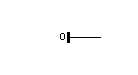
\includegraphics{init0}}
\]

In the same manner, the \verb#hadamard# gate is applied to the newly
created \verb#qubit# and the result is stored in the variable
\verb#q0#. Similarly, another \verb#qubit# is initialized in the state
$\ket{0}$ and stored in the variable \verb#q1#. The rest of the code
is straightforward. A \verb#cnot# gate is applied to the pair
\verb#(q1,q0)# and the pair is then returned.  Note that the pair
\verb#(q0,q1)# \emph{must} be returned as the end of the box
definition to respect the strict linearity of Proto-Quipper. The
hypothetical code where \verb#q0, q1# are not returned would generate
a type error. Finally, every top-level expression in the body of the
module must be terminated by ``\verb#;;#''.

\subsection{Shorthand notations}

In the code of the module \verb#Bell# above, we saw several uses of
the \verb#let# binder. In addition to binding a value to a variable,
the \verb#let# construct also introduces let-polymorphism (an integral
part of all the ML-based languages). Moreover, Proto-Quipper permits
arbitrary \emph{patterns} to be used in place of variables in
bindings. These are defined by the following grammar:
\begin{center}
\begin{tabular}{rrcl}
  $\mathtt{Pattern}$& $p_1 \dots p_n$ & ::= & $x$ \\
                     &                & $|$ & $(p_1, \dots, p_n)$ \\
		     &                & $|$ & $()$
\end{tabular}
\end{center}
As is common in functional programming languages, we introduce shorthand notations to simplify the code. Figure~\ref{sugar} lists the notations introduced in Proto-Quipper. 

\begin{figure}[!ht]
\begin{compactitemize}
\item \verb#let p = a in b#:\\ Binds the variables of the pattern 
  \verb#p#.
\item \verb#p <- a; b#:\\ Equivalent to \verb#let p = a in b#.
\item \verb#p <-* a; b#: \\ Equivalent to \verb#let p = a p in b#.
  Here, \verb#a# must be a function.
\item  \verb#fun p -> a#: \\ Equivalent to
                                \verb#fun x -> let p = x in a#.
\item  \verb#fun x y z -> a#: \\ Equivalent to
                                \verb#fun x -> fun y -> fun z -> a#.
\item  \verb#let f x y z = a in b#: \\ Equivalent to
  \verb#let f = (fun x y z -> a) in b#.
\end{compactitemize}
\caption{Syntactic sugar.}
\label{sugar}
\end{figure}

\subsection{The Quantum Fourier Transform on three qubits}

With the help of the shorthand notations introduced above, we can write 
larger programs. For example, an implementation of the Quantum Fourier 
Transform on three qubits is given in Figure~\ref{fig-qft3}.
\begin{figure}[!ht]
\begin{splitcode}
\begin{verbatim}
box[qubit * qubit * qubit] (
  fun (q0, q1, q2) ->
    q2 <-* hadamard;
    (q2, q1) <-* cphase 2;
    q1 <-* hadamard;
    (q2, q0) <-* cphase 4;
    (q1, q0) <-* cphase 2;
    q0 <-* hadamard;
    (q0, q1, q2)
) ;;
\end{verbatim}
  \split \scalebox{1.4}{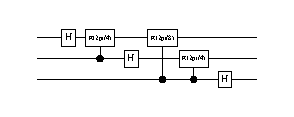
\includegraphics{qft3}}
\end{splitcode}
\caption{An implementation of the Quantum Fourier
Transform on three qubits}
\label{fig-qft3}
\end{figure}
This code illustrates the usefulness of the \verb#p <-* a# notation,
since it is often convenient to store the output of a quantum gate in
a variable of the same name as that of the input. Also note that the
type annotation in \verb#box# is $\qutt\ttt\qutt\ttt\qutt$, rather
than $\qutt\ttt(\qutt\ttt\qutt)$ or $(\qutt\ttt\qutt)\ttt\qutt$.
This is because our implementation of Proto-Quipper allows the use
unparenthesized tuples of arbitrary size.

\subsection{Interactive mode}

If multiple files are passed as arguments to Proto-Quipper, they 
are sequentially executed. If no argument file is given, Proto-Quipper 
enters its interactive mode:
\begin{verbatim}
$ ./ProtoQuipper
### Proto-Quipper -- Interactive Mode ###
# 
\end{verbatim}
In interactive mode, all commands must end with \verb#;;#. This mode accepts:
\begin{compactitemize}
  \item import statements, e.g., \verb#import Gates ;;#,
  \item type definitions, e.g., 
\begin{verbatim}
type list a = Nil | Cons of a * list a ;;
\end{verbatim} 
    and
  \item top-level declarations, e.g., \verb#let x = 1 ;;# or \verb#1+1 ;;#.
\end{compactitemize}
In addition, it is possible to enter commands for the
interpreter. These always start with a \verb#:#. The possible commands are:
\begin{compactitemize}
  \item \verb#:help# --- shows a list of available commands;
  \item \verb#:exit# --- quits the interactive mode;
  \item \verb#:path# $\synarg{dir}$ --- adds a directory to the
    current module path;
  \item \verb#:type# $\synarg{exp}$ --- shows the type of an expression;
  \item \verb#:context# --- lists the currently declared variables;
  \item \verb#:display# --- displays the current top-level circuit.
\end{compactitemize}
Commands can also be abbreviated, for example \verb#:h# or \verb#:c#.

\subsection{Extensions}

The extensions discussed here were introduced in
Section~\hyperref[sec-extensions]{\ref*{sec-extensions}}.

\subsubsection{Polymorphism}

The let-bindings are always assumed to be polymorphic. For example, the 
function:
\begin{verbatim}
let double f q = f (f q) ;;
\end{verbatim}
can be used as follows:
\begin{verbatim}
box[qubit * qubit] (fun (q, r) ->
  q <- double not q;
  (q, r) <- double cnot (q, r);
  (q, r)
) ;;
\end{verbatim}
The first occurrence of \verb#double# has the type 
\begin{verbatim}
!(qubit -> qubit) -> qubit -> qubit,
\end{verbatim}
while the second occurrence has type 
\begin{verbatim}
!(qubit * qubit -> qubit * qubit) -> 
              qubit * qubit -> qubit * qubit.
\end{verbatim}

\subsubsection{Algebraic types, integers and lists}

In the lambda calculus, sum types $A+B$ are usually introduced with
constructors $\leftx : A\to A+B$ and $\rightx : B\to A+B$ and an
operator for case distinctions. This is not particularly
user-friendly. Proto-Quipper therefore provides algebraic types, which
can be seen as a generalization of sum types. The definitions of such
types have to be placed at the beginning of the source file,
immediately following the \verb#import# statements. These definitions
follow the pattern:
\begin{verbatim}
type typename [a b ..] =
    Datacon1 [of T1]
  | Datacon2 [of T2]
  ..
  | DataconN [of TN]
\end{verbatim}
where \verb#a#, \verb#b#, \ldots are type variables and \verb#T1#, \ldots, 
\verb#TN# are type expressions possibly involving the variables \verb#a#, 
\verb#b#, \ldots In particular:
\begin{compactitemize}
  \item The name of the type must start with a lower case character.
  \item The type is followed by zero or more type arguments.
  \item The name of the data constructors starts with an upper case
  character. Each data constructor can take one argument type, introduced 
  by \verb#of#.
  \item Moreover, all the types defined in the same module are assumed
  to be mutually recursive.
\end{compactitemize}
For example, the type of lists included in the module \verb#List# has the 
definition
\begin{verbatim}
type list a =
    Nil
  | Cons of a * list a
\end{verbatim}
Since lists are a very common data structure, special notation has been introduced in the syntax to simplify the writing and manipulation of lists. 
These notations can be used in either expressions or patterns. They are:
\begin{center}
\begin{tabular}{ll}
  \verb#[]#               & for ~ \verb#Nil# \\
  \verb#x:xs#             & for ~ \verb#Cons (x, xs)# \\
  \verb#[x1, ..., xn]# & for ~ 
                            \verb#Cons (x1, ... Cons (xn, Nil) ...)#
\end{tabular}
\end{center}

\subsubsection{Recursion}

Recursive functions can be defined as follows:
\begin{verbatim}
let rec f x y z = a in b
\end{verbatim}
In Proto-Quipper, only functions may be recursively defined. In this
respect, Proto-Quipper differs from Haskell since the latter allows
recursive values like lists of infinite size. This is because
Proto-Quipper follows a strict evaluation strategy (arguments to
functions are evaluated immediately), whereas Haskell follows a lazy
strategy (arguments are evaluated only as needed).

\subsection{The Quantum Fourier Transform}

With the extensions given in the previous subsection, we can write an 
algorithm for the Quantum Fourier Transform for quantum registers encoded 
as lists of qubits. The QFT is now defined as a recursive function that 
inputs and outputs a list of qubits.

We need to import the \verb#List#, \verb#Gates# and \verb#Core# modules. 
The \verb#List# module contains, among other things, the function \verb#sf_last#. Its type is:
\begin{verbatim}
val sf_last <: !(list a -> (a, list a))
\end{verbatim}
This function inputs a list and returns returns its last element. To
satisfy linearity, it also returns the rest of the list. The module
\verb#Core# provides basic integer operations including
\verb#+#, \verb#^#, \verb#-#, \verb#*#, etc. 

The implementation of the algorithm is shown in Figure~\ref{fig-qft}.
It is also contained in the file \verb#qft.qp#.

\begin{figure}[!ht]
\begin{verbatim}
import Core
import Gates
import List

-- Apply the nth phase gate to each qubit of the list, 
-- controlled by a parameter.
let rec appphase n q qn =
  match qn with
   [] -> (q, [])
 | q0:qr ->
     (q, qr) <- appphase (n+1) q qr;
     (q0, q) <-* cphase (2 ^ n);
     (q, q0:qr)
;;

-- Quantum Fourier Transform.
let rec qft qreg =
  match qreg with
    [] -> []
  | q:reg ->
      (qn, qn1) <- sf_last (q:reg);
      qn1 <- qft qn1;
      (qn, qn1) <- appphase 1 qn qn1;
      qn <-* hadamard;
      qn:qn1
;;
\end{verbatim}
\[\scalebox{1.2}{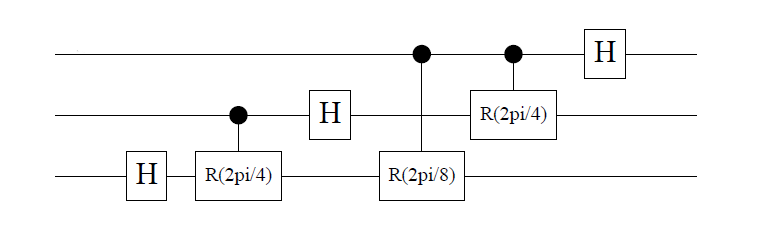
\includegraphics{qft}}
\]

  \caption{An implementation of the Quantum Fourier Transform on lists
    of qubits}
  \label{fig-qft}
\end{figure}
